\chapter{ Conception et environnement Technique} 
 \minitoc
 \newpage
 \counterwithin{figure}{chapter}

 \section{Introduction}
 Ce chapitre présente les éléments techniques et conceptuels ayant guidé la réalisation de la solution. Il introduit le cadre de développement ainsi que les principaux choix adoptés. La section \ref{sec:Environnement de travail} décrit l'environnement de travail et les technologies utilisées. La section \ref{sec:Architecture générale de l'application} présente l'architecture générale du système. La section \ref{sec:Conception technique et modélisation multidimensionnelle} est consacrée à la conception technique et à la modélisation du système, tandis que la section \ref{sec:Conception de l'interface des utilisateurs } traite de la conception de l'interface utilisateur. Enfin, une synthèse des choix effectués clôt ce chapitre afin de préparer la phase d'implémentation.
 \section{Environnement de travail}
 \label{sec:Environnement de travail}
L'environnement de travail regroupe tous les outils, langages et frameworks utilisés pour concevoir, développer et tester une application. Il joue un rôle essentiel pour assurer l'efficacité, la cohérence et la qualité du projet.


\subsection{Outils de développement et modélisation}

\noindent
\begin{minipage}{0.55\textwidth}
\raggedright
\textbf{UML (Unified Modeling Language):} Le Langage de Modélisation Unifié (voir figure \ref{fig:uml_logo}), de l'anglais Unified Modeling Language (UML) \cite{uml_spec}, est un langage de modélisation graphique à base de pictogrammes conçu comme une méthode normalisée de visualisation dans les domaines du développement logiciel et en conception orientée objet.
\end{minipage}
\hfill
 \begin{minipage}{0.4\textwidth}
        \centering
        
\includegraphics[width=0.8\textwidth]{project/images/UML_logo.svg.png}

       \captionof{figure}{Logo UML}
       \label{fig:uml_logo}
    \end{minipage}

\noindent
\begin{minipage}{0.55\textwidth}
\raggedright
\textbf{Visual Studio Code :} (ou VS Code) \cite{vscode_docs}, est un éditeur de code source gratuit, léger et performant, développé par Microsoft. Il est très populaire pour le développement web et logiciel grâce à sa rapidité, la coloration syntaxique, la saisie semi-automatique intelligente, les extraits de code, les outils de restructuration de code et le contrôle de version Git intégré (voir figure \ref{fig:vscode_logo}).
\end{minipage}
\hfill
 \begin{minipage}{0.3\textwidth}
        \centering
        
\includegraphics[width=0.7\textwidth]{project/images/image.png}

       \captionof{figure}{logo VsCode}
       \label{fig:vscode_logo}
    \end{minipage}
    
\noindent
\begin{minipage}{0.55\textwidth}
\raggedright
\textbf{Figma :} \cite{figma_docs} est une plateforme de conception graphique vectorielle et de prototypage basée sur le cloud (voir figure \ref{fig:figma_logo}), principalement utilisée pour créer des interfaces utilisateur (UI) et des expériences utilisateur (UX) de sites web et d'applications mobiles. Il permet la collaboration en temps réel, facilitant le travail d'équipe, le design system et le passage de relais aux développeurs.
\end{minipage}
\hfill
 \begin{minipage}{0.3\textwidth}
        \centering
        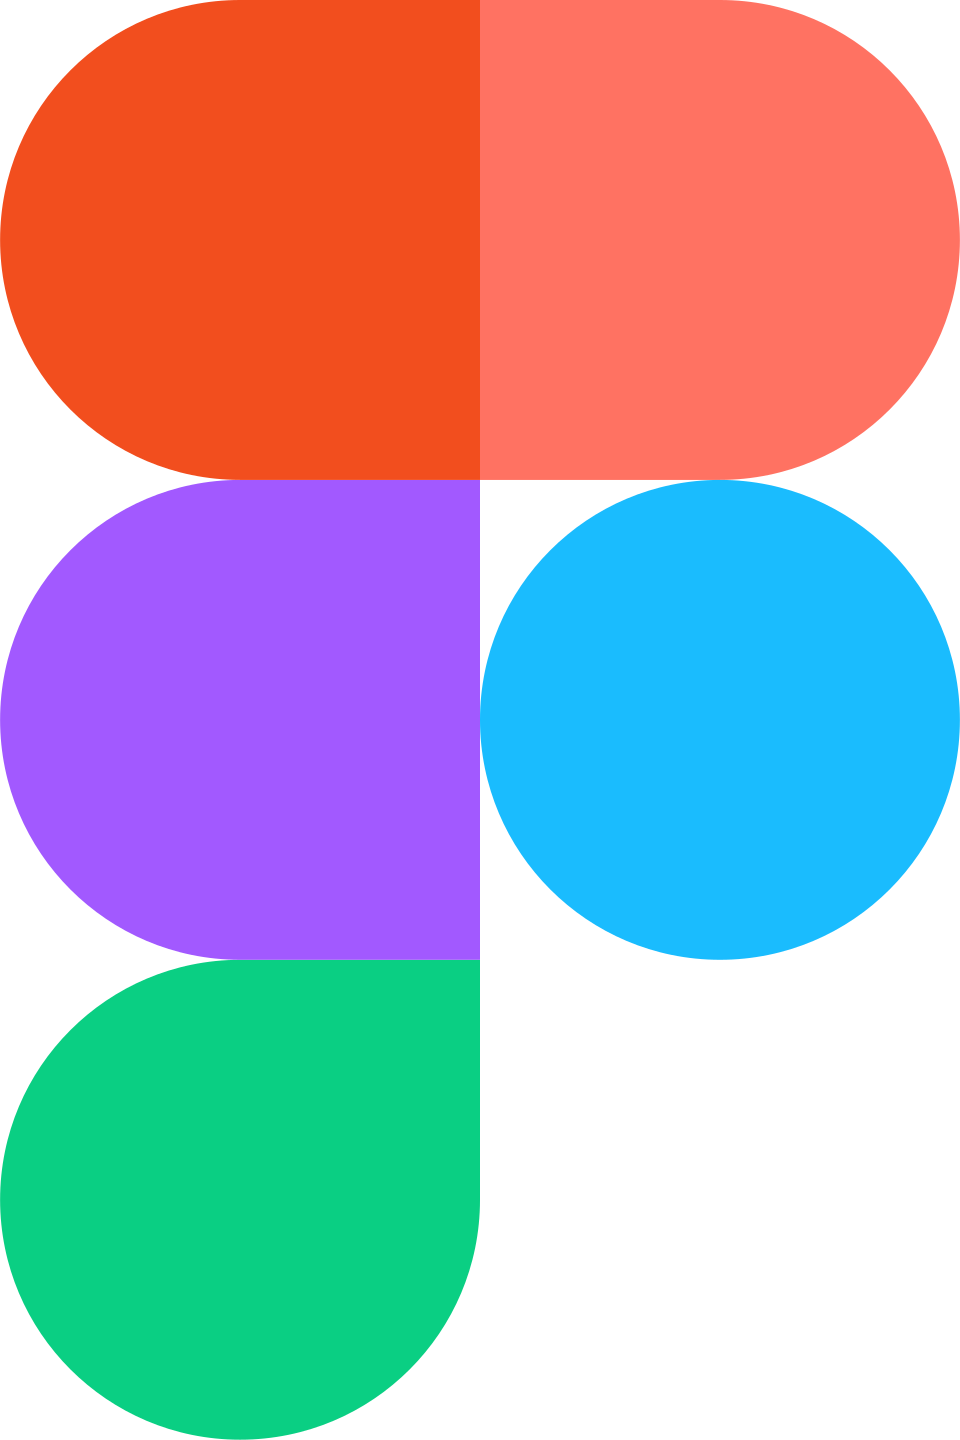
\includegraphics[width=0.5\textwidth]{project/images/Figma-logo.svg.png}

       \captionof{figure}{Logo Figma}
       \label{fig:figma_logo}
    \end{minipage}

\noindent
\begin{minipage}{0.55\textwidth}
\raggedright
\textbf{GitHub:} \cite{github_docs} est une plateforme de développement collaboratif qui permet aux développeurs de stocker, gérer et suivre les modifications de leur code source en utilisant Git, un système de gestion de versions distribué (voir figure \ref{fig:github_logo}).
\end{minipage}
\hfill
 \begin{minipage}{0.3\textwidth}
        \centering
        
\includegraphics[width=0.7\textwidth]{project/images/25231.png}

       \captionof{figure}{ Logo GitHub}
       \label{fig:github_logo}
    \end{minipage}

\noindent
\begin{minipage}{0.55\textwidth}
\raggedright
\textbf{Postman :} \cite{postman_docs} est un outil de développement d'API qui permet aux développeurs de tester, déboguer et documenter les API de manière efficace. Son interface conviviale simplifie le processus de test des requêtes HTTP et de collaboration au sein des équipes (voir figure \ref{fig:postman_logo}).
\end{minipage}
\hfill
 \begin{minipage}{0.3\textwidth}
        \centering
        
\includegraphics[width=0.7\textwidth]{project/images/unnamed.png}

 \captionof{figure}{ Logo Postman}
       \label{fig:postman_logo}
    \end{minipage}
    

\subsection{Langages de programmation}
Cette section présente les principaux langages de programmation utilisés dans le développement du projet.

\noindent
\begin{minipage}{0.55\textwidth}
\raggedright
\textbf{JavaScript :} \cite{javascript_mdn} est un langage de programmation interprété (voir figure \ref{fig:javascript_logo}), dynamique et polyvalent, principalement utilisé pour rendre les pages web interactives. Il est aujourd'hui un pilier du développement web moderne et fonctionne aussi bien côté client (navigateur) que côté serveur via Node.js.
\end{minipage}
\hfill
 \begin{minipage}{0.3\textwidth}
        \centering
        
\includegraphics[width=0.7\textwidth]{project/images/img_javascript_480.jpg}

 \captionof{figure}{Logo Js}
       \label{fig:javascript_logo}
    \end{minipage}
    
\noindent
\begin{minipage}{0.55\textwidth}
\raggedright
\textbf{TypeScript :} \cite{typescript_docs} représente l'évolution moderne de JavaScript, apportant un système de typage statique qui renforce considérablement la robustesse et la maintenabilité du code (voir Figure \ref{fig:typescript_logo}).
\end{minipage}
\hfill
 \begin{minipage}{0.3\textwidth}
        \centering
        
\includegraphics[width=0.8\textwidth]{project/images/typescript.png}

 \captionof{figure}{Logo TypeScript}
       \label{fig:typescript_logo}
    \end{minipage}

\noindent
\begin{minipage}{0.55\textwidth}
\raggedright
\textbf{Python :} \cite{python_docs} est un langage de programmation de haut niveau (voir figure \ref{fig:python_logo}), interprété et orienté objet, reconnu pour sa syntaxe intuitive et facile à lire. Open source, il est largement adopté pour des domaines variés tels que le développement web, la science des données, l'intelligence artificielle et l'automatisation.
\end{minipage}
\hfill
 \begin{minipage}{0.3\textwidth}
        \centering
        
\includegraphics[width=0.7\textwidth]{project/images/Python-logo-notext.svg.png}
        \captionof{figure}{Logo Python}
        \label{fig:python_logo}
    \end{minipage}


\subsection{Framework et technologies utilisé}
\noindent
\begin{minipage}{0.55\textwidth}
\raggedright
\textbf{Next.js :} \cite{nextjs_docs} est un framework moderne basé sur React, conçu pour faciliter le développement d'applications web complètes (full-stack). Il permet aux développeurs de créer des interfaces utilisateur dynamiques en s'appuyant sur les composants React, tout en bénéficiant de fonctionnalités avancées et d'optimisations intégrées (voir figure \ref{fig:nextjs_logo}).
\end{minipage}
\hfill
 \begin{minipage}{0.3\textwidth}
        \centering
        
\includegraphics[width=0.7\textwidth]{project/images/images (5).png}

 \captionof{figure}{Logo NextJs}
        \label{fig:nextjs_logo}
    \end{minipage}

\noindent
\begin{minipage}{0.55\textwidth}
\raggedright
\textbf{NestJS :} \cite{nestjs_docs} est un framework backend moderne basé sur Node.js et TypeScript (voir figure \ref{fig:nestjs_logo}), offrant une architecture modulaire et évolutive pour le développement d'applications serveur. Il fournit des fondations robustes pour construire des API REST, des microservices ou toute logique métier côté serveur, tout en facilitant la maintenabilité et l'organisation du code.
\end{minipage}
\hfill
 \begin{minipage}{0.3\textwidth}
        \centering
        
\includegraphics[width=0.7\textwidth]{project/images/images (6).png}

 \captionof{figure}{Logo NestJs}
        \label{fig:nestjs_logo}
    \end{minipage}

\noindent
\begin{minipage}{0.55\textwidth}
\raggedright
\textbf{Chart.js :} \cite{chartjs_docs} est une bibliothèque JavaScript open-source (voir figure \ref{fig:chartjs_logo}) qui permet de créer facilement des graphiques interactifs et visuels dans une application web. Elle utilise le canevas HTML5 pour dessiner différents types de graphiques (barres, lignes, camemberts, etc.) et offre des options de personnalisation pour représenter clairement des données.
\end{minipage}
\hfill
 \begin{minipage}{0.3\textwidth}
        \centering
        % TODO: Add Chart.js logo image file (chartjs-logo.png) to project/images/
        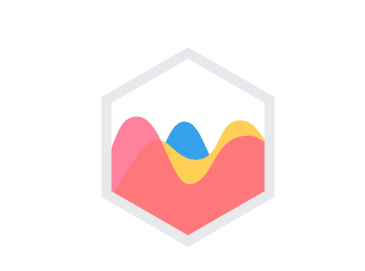
\includegraphics[width=\textwidth]{project/images/chartjs-logo.png}

 \captionof{figure}{Logo Chartjs}
        \label{fig:chartjs_logo}
    \end{minipage}

\subsection{Base de données}
\noindent
\begin{minipage}{0.55\textwidth}
\raggedright
\textbf{PostgreSQL:} \cite{postgresql_docs} est un système de gestion de base de données relationnelle orientée objet, open source et performant, capable de gérer des données complexes. Il privilégie la conformité SQL et l'extensibilité. De plus, il est adapté aux charges de travail OLAP (Online Analytical Processing), ce qui permet d'effectuer des analyses et des traitements avancés sur de grands volumes de données (voir figure \ref{fig:postgressql_logo}).
\end{minipage}
\hfill
 \begin{minipage}{0.3\textwidth}
        \centering
        
\includegraphics[width=0.7\textwidth]{project/images/elephant.png}

 \captionof{figure}{Logo PostgresSql}
        \label{fig:postgressql_logo}
    \end{minipage}
\newline

 \section{Architecture générale de l'application}
  \label{sec:Architecture générale de l'application}
 L'architecture désigne la structure technique qui organise les différents composants de l'application (frontend, backend, base de données, services externes) ainsi que leurs interactions. Elle définit la circulation des données, les modalités de communication entre les composants et l'emplacement ou le mode d'exécution de chaque élément. Dans cette section, nous présentons l'architecture logicielle de notre application. La figure \ref{fig:placeholder} illustre l'architecture générale retenue, laquelle est structurée en trois parties principales. \newline

\begin{figure}[H]
     \centering
     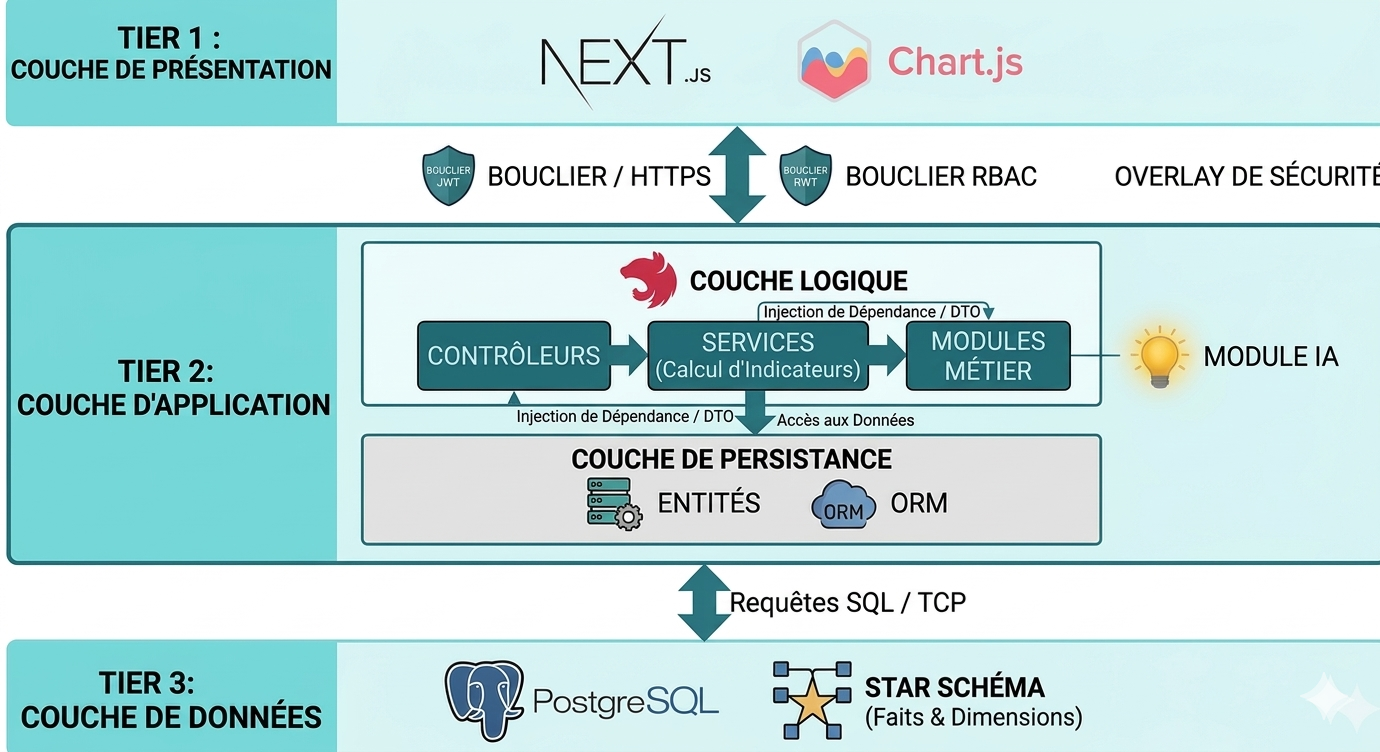
\includegraphics[width=0.8\linewidth]{project/images/Gemini_Generated_Image_jsvpksjsvpksjsvp.png}
     \caption{architecture generale}
     \label{fig:placeholder}
 \end{figure}
 \vspace{0.8cm}
 
\textbf{Tier 1 : Couche de Présentation (Front-end)}\newline
Il représente les interfaces de l'application, c'est-à-dire les éléments avec lesquels l'utilisateur peut interagir. \newline
\textbf{Tier 2 : Couche Application (Back-end)}\newline
Il englobe les fonctionnalités de l'application et leur implémentation. Il est invisible pour les utilisateurs de l'application, mais il assure le dynamisme de celle-ci.

\textbf{communication et securité:} La communication entre le frontend et le backend se fait via des API REST, utilisant des requêtes HTTP pour échanger des données au format JSON. Pour garantir la sécurité de ces échanges, nous avons mis en place une couche de sécurité qui valide les jetons d'authentification (JWT) et vérifie les droits d'accès (RBAC) avant de permettre l'accès aux ressources protégées du backend.

\textbf{Couche logique :} 
représente la partie centrale de l'application où sont implémentées les règles métier. Elle est responsable du traitement des données, de l'exécution des opérations et de la prise de décisions en fonction des besoins fonctionnels.

\textbf{Couche persistence :} Utilise un ORM (Object-Relational Mapping) pour faire le pont entre le code et la base de données, assurant une manipulation fluide des Entities.\newline
\textbf{Tier 3 : Couche de Données (Database)}\newline
Elle englobe la base de données ainsi que les différents mécanismes permettant de manipuler les données de façon sécurisée et efficace.
\newline

\section{Conception technique et modélisation multidimensionnelle}
\label{sec:Conception technique et modélisation multidimensionnelle}
\subsection{Diagramme de classes}
Dans cette section, nous allons explorer la structure logique de la plateforme à travers son diagramme de classes. Ce diagramme permet de visualiser les principales entités du système, leurs attributs et méthodes essentiels, ainsi que les relations qui les lient, offrant ainsi une vue d'ensemble claire de l'architecture du projet.

La figure \ref{fig:diagramme de classe} présente cette modélisation et illustre comment les différentes classes interagissent pour assurer le fonctionnement cohérent de la plateforme.

\begin{figure}[H]
  \centering
    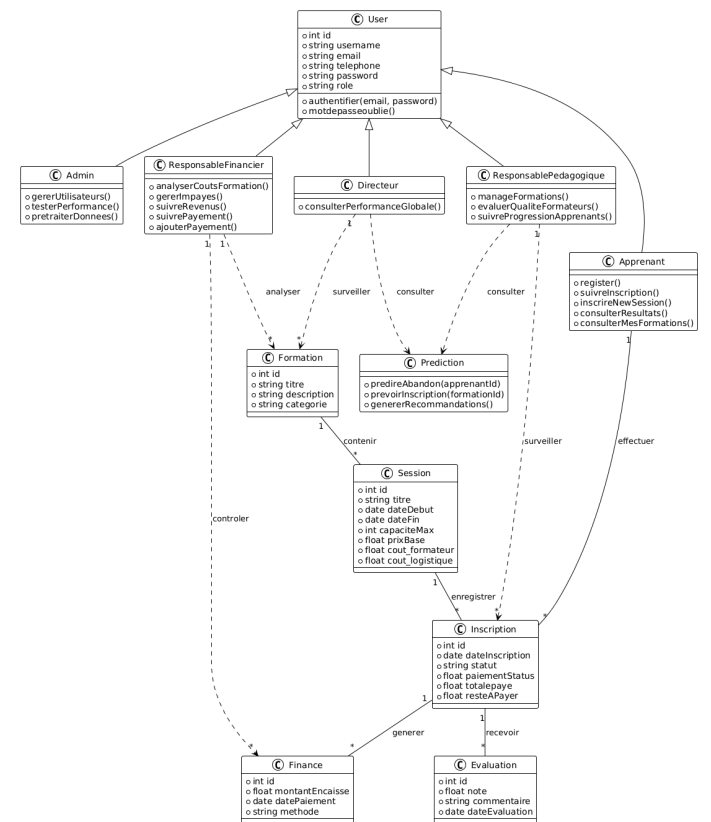
\includegraphics[scale=0.8]{project/images/diagClasse.png}
  \caption{ Diagramme de classe}
  \label{fig:diagramme de classe}
\end{figure}

\subsection{Modélisation décisionnelle}
La modélisation multidimensionnelle est l'étape clé pour structurer les données afin de faciliter l'analyse. Le système repose sur une architecture ROLAP, implémentée à l’aide d’une base de données relationnelle PostgreSQL, en s’appuyant sur un schéma en constellation pour optimiser les requêtes analytiques.

\textbf{ Les Dimensions}\newline Les dimensions représentent les axes d'analyse 

Dim-Temps: Permet d'analyser les données par année, semestre, mois et jour.

Dim-Apprenants: Regroupe les informations sur les profils inscrits (niveau, ville, etc.).

Dim-Formations: Contient les détails des programmes proposés.

Dim-Formateurs: Identifie les intervenants et leurs expertises.

Dim-Sessions: Précise le cadre temporel et physique (ou virtuel) des cours.

\textbf{ Les Faits}\newline
Les faits contiennent les mesures quantitatives (les indicateurs de performance ou KPIs).

Faits-Inscriptions : Analyse le volume des nouveaux inscrits et les flux d'admission.

Faits-Performances : Suit les résultats pédagogiques (notes, taux de réussite).

Faits-Finances : Centralise les données monétaires (revenus, impayés, CA).

Le choix du schéma en étoile se justifie par la simplicité des jointures. Contrairement à un schéma en flocon, il réduit le nombre de tables à interroger, ce qui accélère la génération des graphiques dans le dashboard final.

\section{Conception de l'interface des utilisateurs }
\label{sec:Conception de l'interface des utilisateurs }
La conception des interfaces a débuté par une approche intégrée combinant l'interface utilisateur (UI) et l'expérience utilisateur (UX), essentielles pour une solution intuitive et efficace.
l'utilisation de Figma pour concevoir les interfaces
avant leur développement s'est révélée cruciale. Cette approche a permis de prototyper rapidement les flux utilisateur, tester les interactions, et optimiser le temps de livraison en identifiant
les besoins essentiels. Cette sous-section détaille ces deux aspects
distincts, en s'appuyant sur des bases théoriques et pratiques adaptées au projet.
\subsection{Conception UI/UX}
\textbf{Interface Utilisateur (UI) }\newline
L'interface utilisateur (UI) constitue le principal point d'interaction avec la plateforme décisionnelle, conçue pour offrir une visualisation claire et intuitive des KPIs. Une hiérarchisation efficace met en avant les indicateurs clés sous forme de cartes, complétées par des graphiques interactifs pour analyser les tendances. la typographie a été définie avec la police Inter, largement utilisée dans le projet pour sa modernité et sa lisibilité, garantissant une présentation claire des
texte, Le choix de la palette de couleurs s'est orienté vers des tons \textit{sage} et \textit{cream}, comme illustré dans la Figure \ref{fig:placeholder3}. Ces couleurs ont été sélectionnées pour leur aspect apaisant et professionnel, favorisant une meilleure lisibilité des informations. Toutefois, ce choix reste évolutif et pourra faire l'objet d'ajustements lors de la phase de réalisation, afin d'améliorer davantage l'expérience utilisateur et l'ergonomie de l'interface.
\begin{figure}[H]
     \centering
     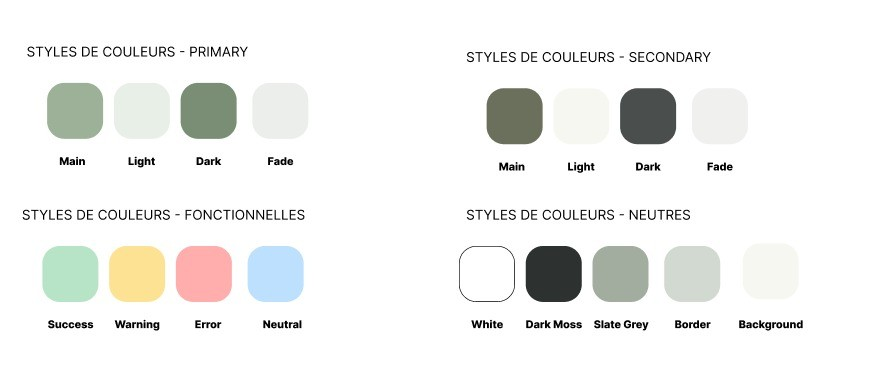
\includegraphics[width=0.8\linewidth]{project/images/WhatsApp Image 2026-03-23 at 9.56.31 PM.jpeg}
     \caption{palette de couleurs suggérée }
     \label{fig:placeholder3}
 \end{figure}
 \vspace{0.8cm}
\textbf{Expérience Utilisateur (UX)}
L'expérience utilisateur (UX) se focalise sur la manière dont les utilisateurs perçoivent et interagissent avec la plateforme décisionnelle, dans le but d'optimiser leur satisfaction et l'efficacité de leur travail. L'organisation de l'information a été pensée pour présenter le contenu et les options de navigation de façon claire et logique, facilitant un accès rapide aux fonctionnalités essentielles. Les interactions sont fluides et cohérentes entre les différents écrans, tandis que les parcours utilisateurs sont conçus pour guider intuitivement l'exploration des données et des KPIs. Ces choix ergonomiques contribuent à une expérience agréable, efficace et adaptée aux besoins d'analyse et de suivi des performances.
\newline

\subsection{Maquettage de l'interface}

Les maquettes présentées dans cette section représentent une première version du design de l'interface.La Figure \ref{fig:placeholder1} montre l'écran de connexion de la plateforme décisionnelle, tandis que la Figure \ref{fig:placeholder2} présente l'interface du Responsable Pédagogique, Elles ont été conçues afin de définir la structure générale des écrans et l'organisation des informations. Des améliorations seront apportées par la suite, notamment en ce qui concerne l'harmonisation et la gradation des couleurs ainsi que l'optimisation de l'ergonomie.

\begin{figure}[H]
     \centering
     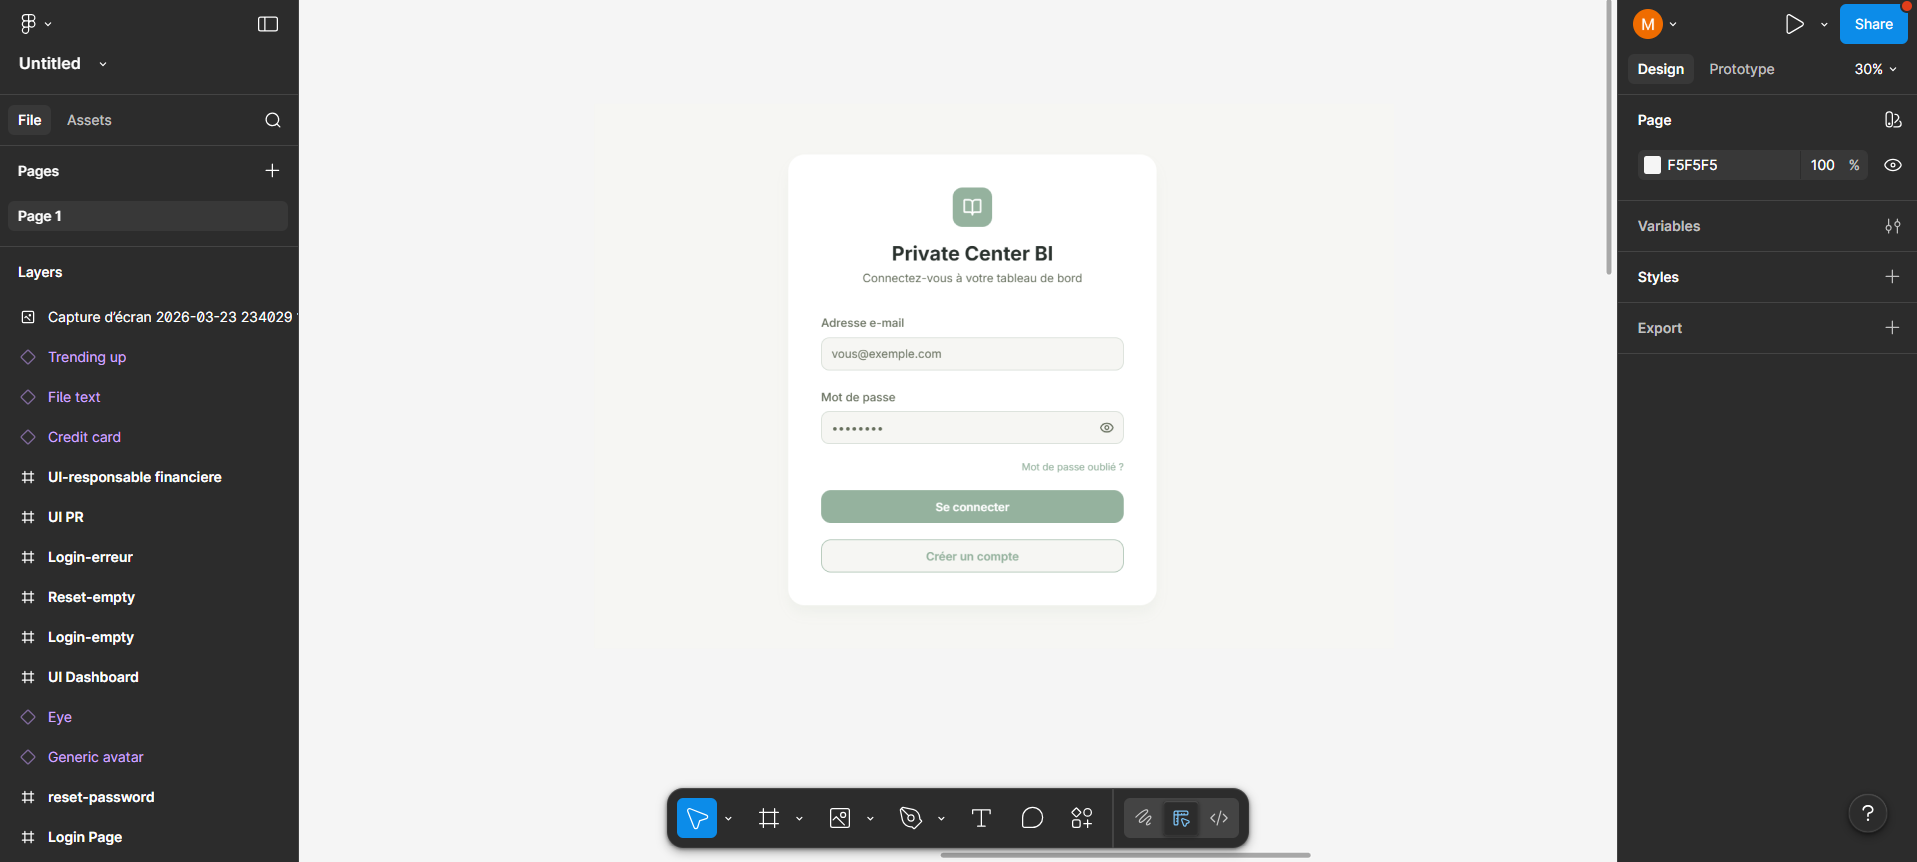
\includegraphics[width=0.8\linewidth]{project/images/Capture d’écran 2026-03-23 234150.png}
     \caption{maquette de l'écran de connexion }
     \label{fig:placeholder1}
 \end{figure}

        \begin{figure}[H]
     \centering
     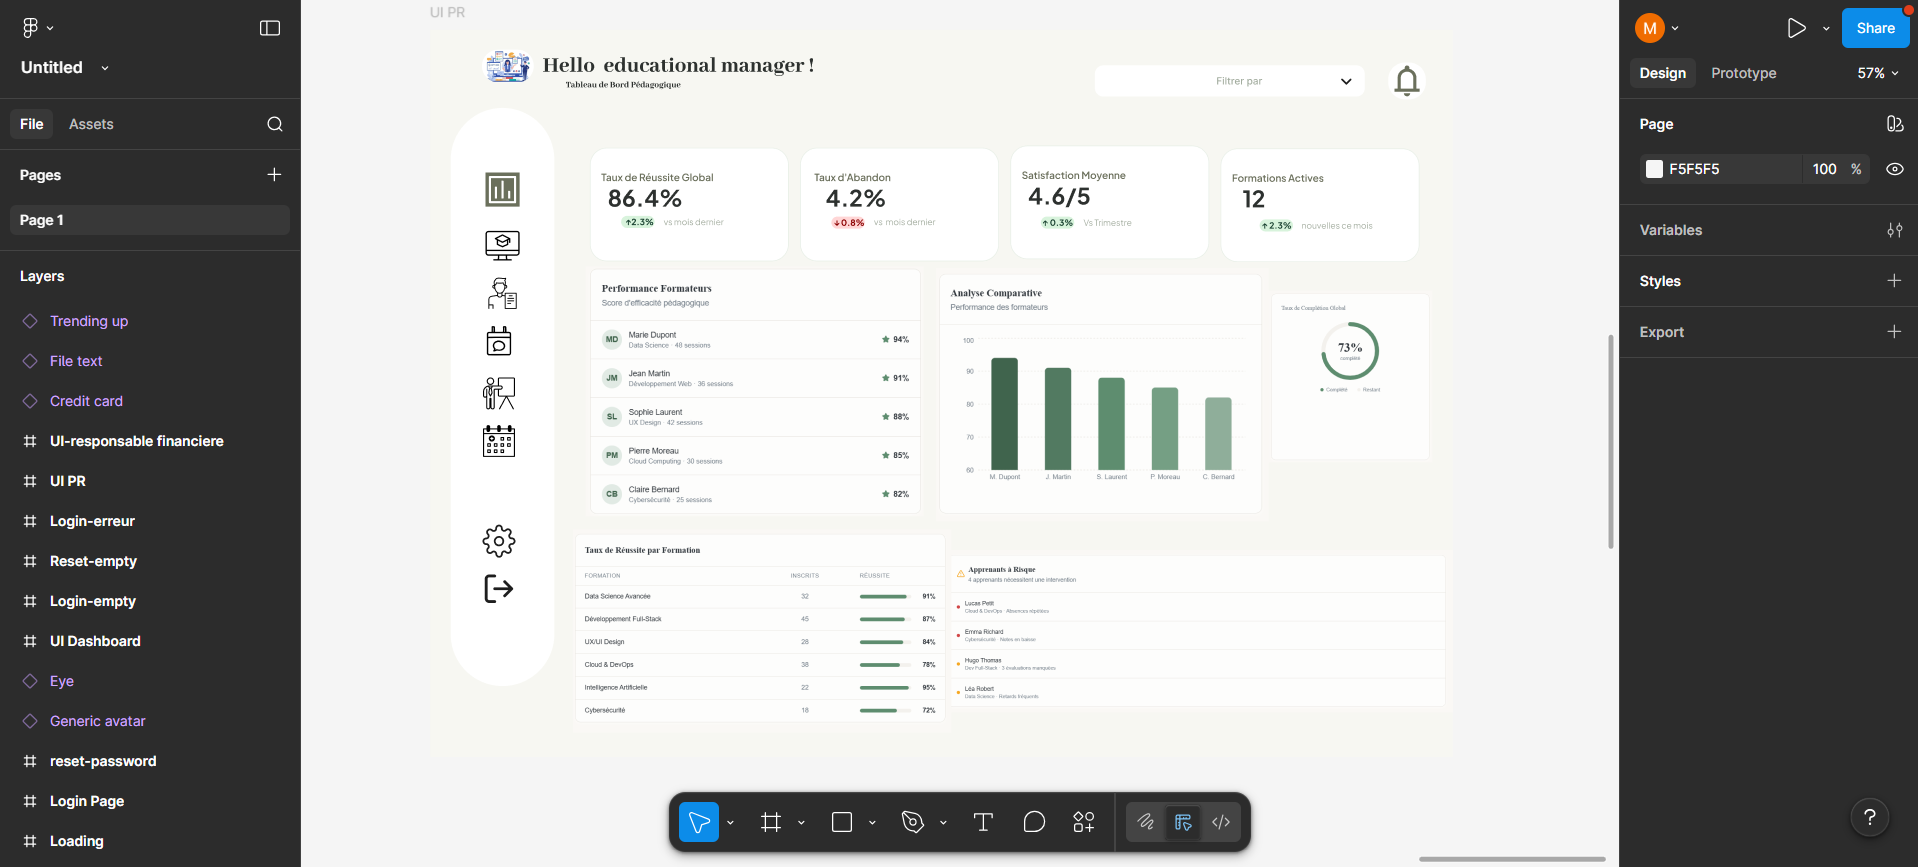
\includegraphics[width=0.8\linewidth]{project/images/Capture d’écran 2026-03-23 232928.png}
     \caption{maquette de l'interface du Responsable Pédagogique}
     \label{fig:placeholder2}
 \end{figure}
 

\section{Conclusion}
En résumé, ce chapitre a permis de définir l'environnement de travail et les technologies choisis pour garantir la performance du système. Nous avons détaillé l'architecture générale ainsi que la conception technique, notamment à travers le diagramme de classes et la modélisation décisionnelle. 
Enfin, l'étude de l'interface utilisateur (UI/UX) et le maquettage ont permis de fixer l'aspect visuel de la plateforme. Ce cadre conceptuel étant validé, nous pouvons maintenant passer à la phase de réalisation de l'application.